\documentclass[xetex,18pt,aspectratio=43]{beamer}

\usepackage{caption}
\usepackage[percent]{overpic}
\usepackage{xecyr}
\usepackage{xunicode}
\usepackage[absolute,overlay]{textpos}
\usepackage{fontspec}
\usepackage{calc}
\usepackage{multicol}
\usepackage{hyperref}
\usepackage{setspace}
\usepackage{tikz}
\usepackage{csquotes}
\usepackage[export]{adjustbox}
%\usepackage[texcoord,grid,gridunit=mm,gridcolor=red!10,subgridcolor=green!10]{eso-pic}
\defaultfontfeatures{Ligatures=TeX}
\setmainfont{Trebuchet MS}
\usepackage{polyglossia}
\setdefaultlanguage[spelling=modern]{russian}
\newfontfamily{\cyrillicfont}{Trebuchet MS}
\newfontfamily{\cyrillicfontsf}{Trebuchet MS}
\newfontfamily{\cyrillicfonttt}{Trebuchet MS}
\newfontface\lserif{Microsoft Sans Serif}

\newcommand\Bigfont{\fontsize{22}{22}\selectfont}
\newcommand\Authorfont{\fontsize{17}{17}\selectfont}
\newcommand\Orgfont{\fontsize{13}{13}\selectfont}

\mode<presentation>
{
  %\usetheme{Boadilla}      % or try Darmstadt, Madrid, Warsaw, ...
  \usecolortheme{default} % or try albatross, beaver, crane, ...
  %\usefonttheme{default}  % or try serif, structurebold, ...
  \setbeamertemplate{navigation symbols}{}
  \setbeamertemplate{caption}[numbered]
  \setbeamertemplate{itemize items}[circle]
  \setbeamerfont{title}{series=\bfseries,parent=structure}
  \setbeamerfont{frametitle}{size=\huge}
} 

\makeatother
\setbeamertemplate{footline}
{
  \leavevmode%
  \hbox{%
  \begin{beamercolorbox}[wd=.35\paperwidth,ht=2.5ex,dp=1ex,center]{author in head/foot}%
    \usebeamerfont{author in head/foot}\insertshortauthor
  \end{beamercolorbox}%
  \begin{beamercolorbox}[wd=.65\paperwidth,ht=2.5ex,dp=1ex,center]{title in head/foot}%
    \usebeamerfont{title in head/foot}\insertshorttitle\hfill
    \insertframenumber{} / \inserttotalframenumber\hspace*{-8ex}
  \end{beamercolorbox}}%
  \vskip0pt%
}
\makeatletter

\title[Страх и отвращение в Санкт-Петербурге]{}
\author[Александр Чистяков, Git in Sky]{}
\date{}

\begin{document}

{ % all template changes are local to this group.
    \setbeamertemplate{navigation symbols}{}
    %\setbeamertemplate{background}[grid][step=10]
    \setbeamertemplate{background}{
\includegraphics[width=\paperwidth,height=\paperheight,keepaspectratio]{img/firstslide.png}}
    \begin{frame}[plain]
      \begin{textblock*}{\framewidth}(0.95cm,3.7cm) % {block width} (coords)
        \Bigfont
          \begin{center}
          Страх и отвращение в Санкт-Петербурге
          \end{center}
      \end{textblock*}
      \begin{textblock*}{\framewidth}(0.95cm,6.7cm) % {block width} (coords)
        \Authorfont
          \begin{center}
          Александр Чистяков
          \end{center}
      \end{textblock*}
      \begin{textblock*}{\framewidth}(0.95cm,7.8cm) % {block width} (coords)
        \Orgfont
          \begin{center}
          Git in Sky
          \end{center}
      \end{textblock*}
     \end{frame}
}


\begin{Large}
\begin{frame}{\ \ \ Несколько слов о себе}
\setstretch{1.2}
\begin{textblock*}{\framewidth-0.8cm}(0.5cm,1.5cm)
\begin{itemize}
  \item Главный инженер в \href{https://gitinsky.com}{\color{blue}{Git in Sky}}
  \item Преподаватель в \href{http://avalon.ru}{\color{blue}{avalon.ru}}
  \item Researcher @ ISST Lab, \href{http://ifmo.ru}{\color{blue}{ITMO}}
  \item Координатор \href{https://meetup.com/DevOps-40}{\color{blue}{встреч}} DevOps-инженеров в Петербурге
  \item Пишу код
\end{itemize}
\end{textblock*}
\end{frame}

\begin{frame}{\ \ \ Слово \enquote{современные}}
\setstretch{1.2}
\begin{textblock*}{\framewidth}(0.8cm,1.5cm)
Что изображено на картинке?\\
{\small (Мы будем говорить о вещах, придуманных 30 и более лет назад)}
\begin{minipage}{\textwidth}
  \centering
  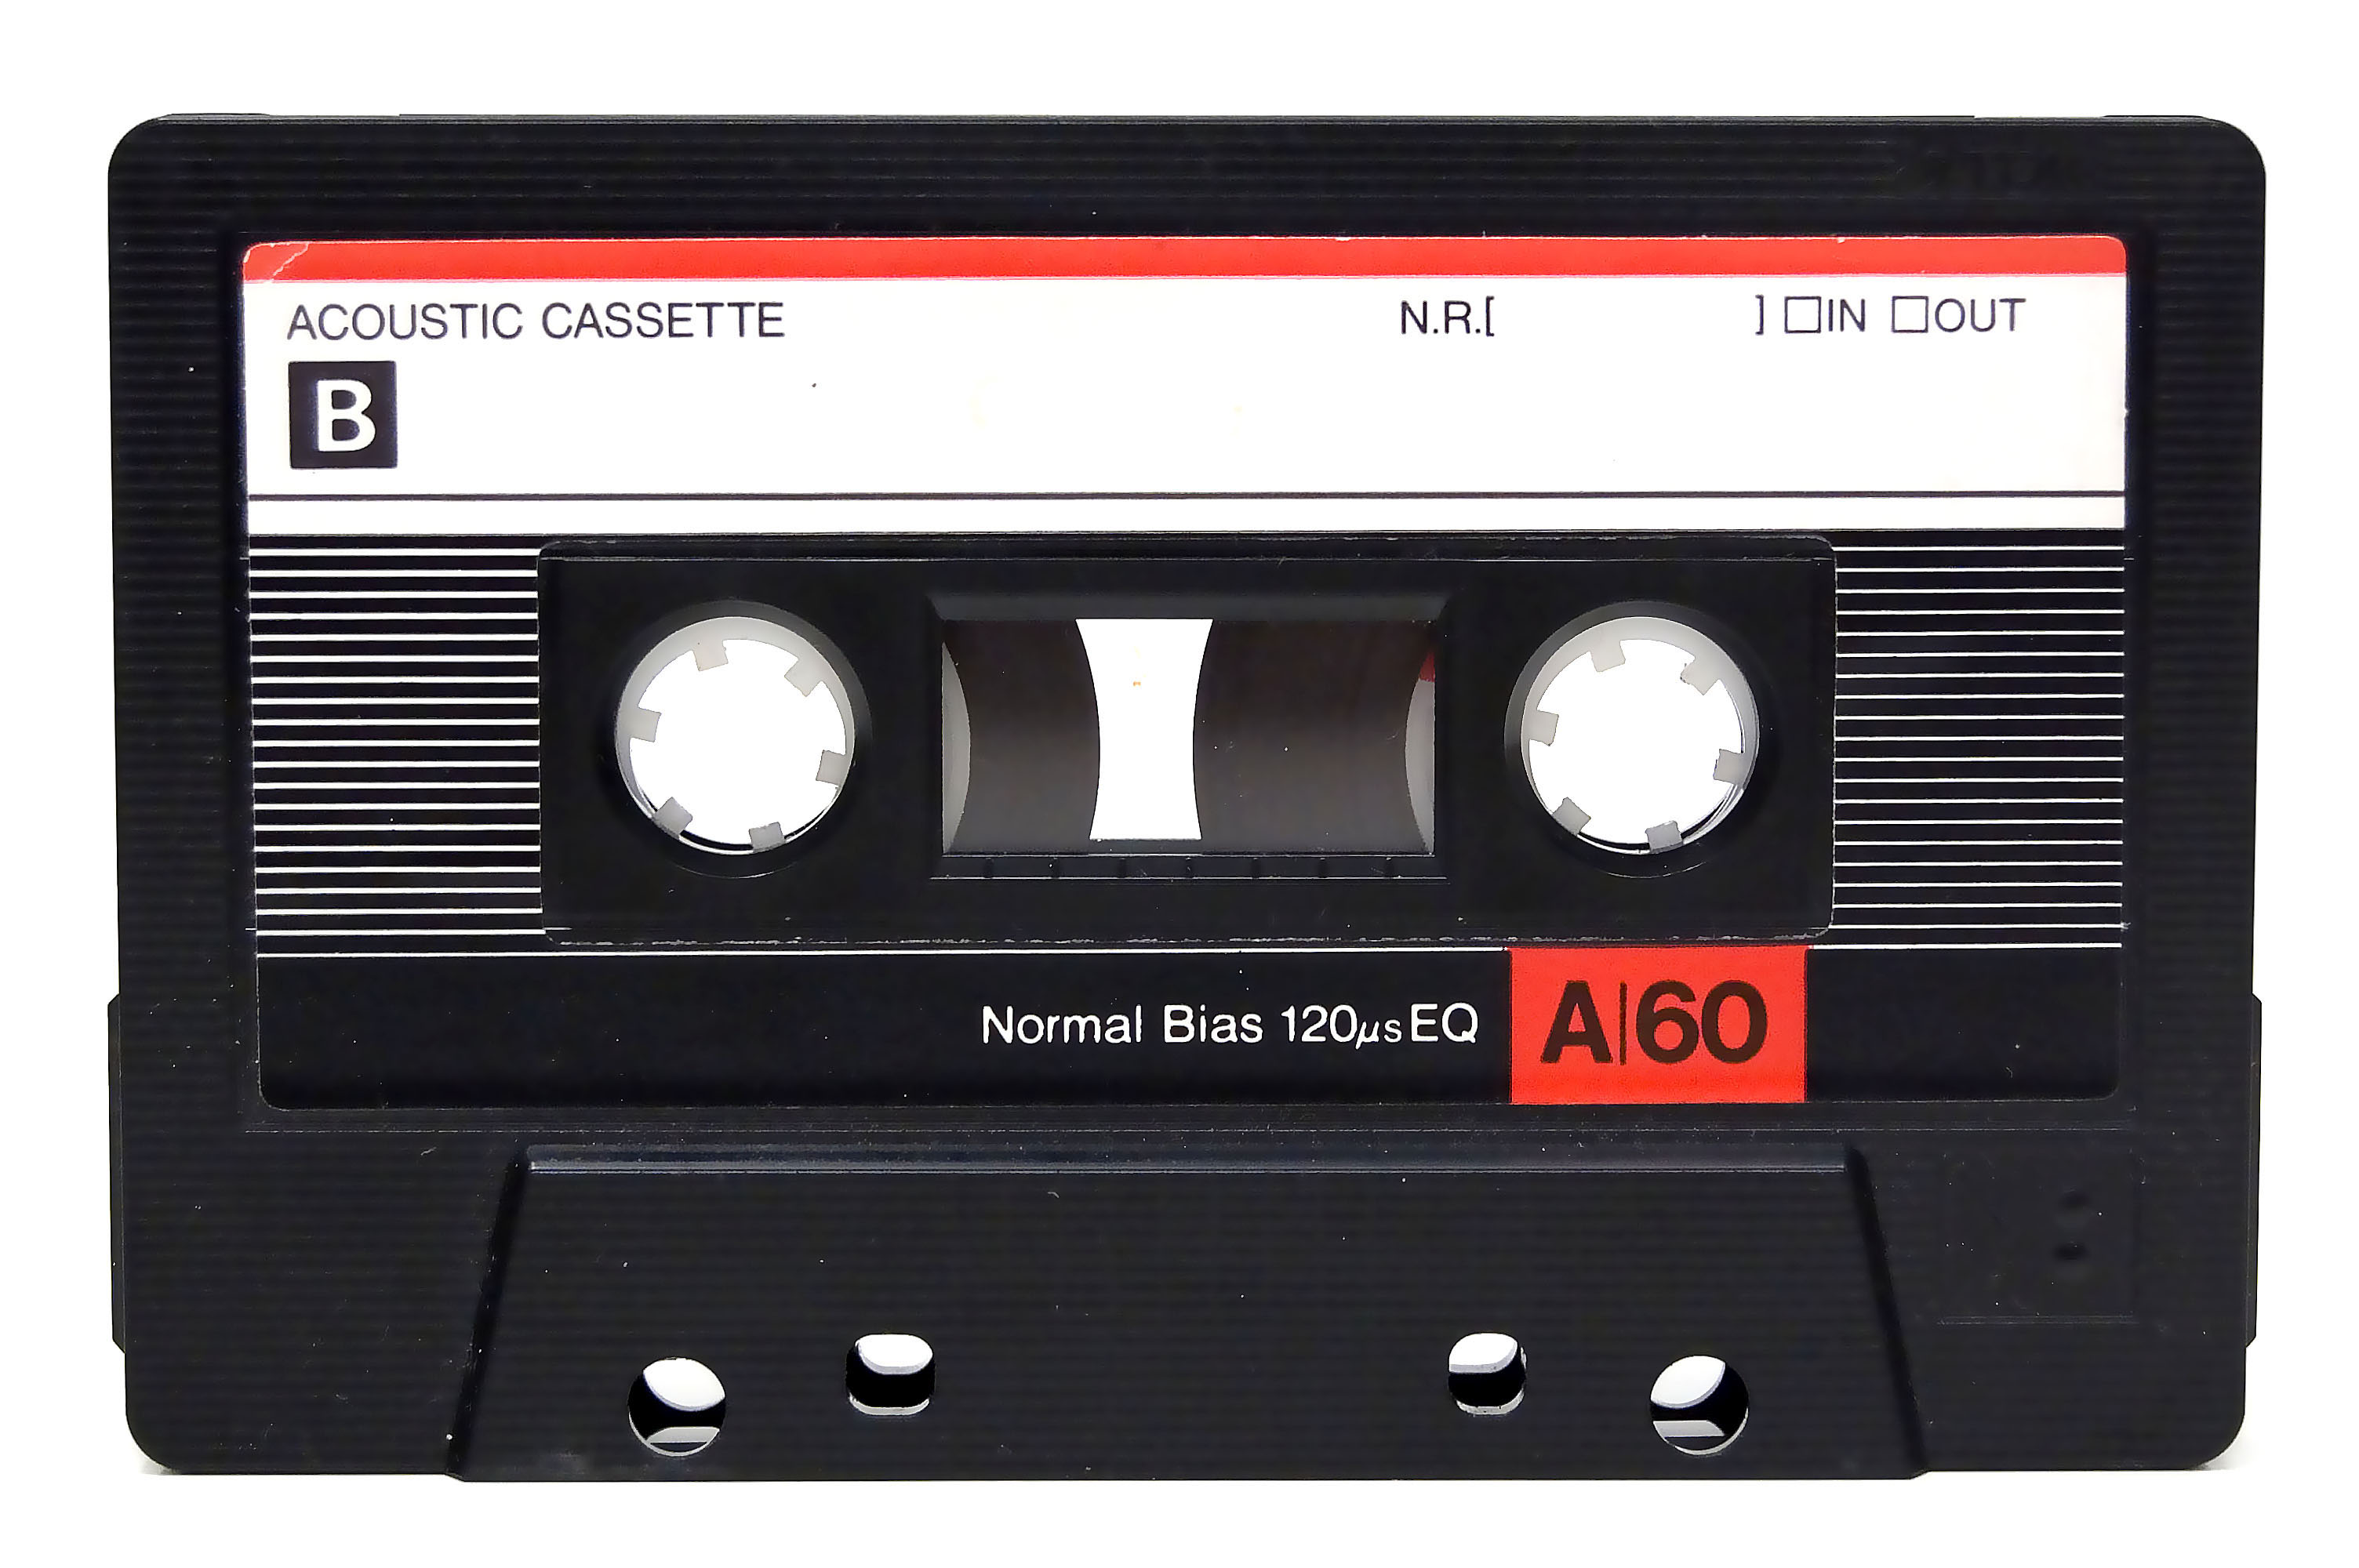
\includegraphics[height=5.5cm]{img/cassette}
\end{minipage}
\end{textblock*}
\end{frame}

\begin{frame}{\ \ \ Немного истории}
\setstretch{1.2}
\begin{textblock*}{\framewidth}(0.8cm,1.5cm)
Носитель информации 30 лет назад\\
{\small (Емкость примерно 200 килобайт)}
\begin{minipage}{\textwidth}
  \centering
  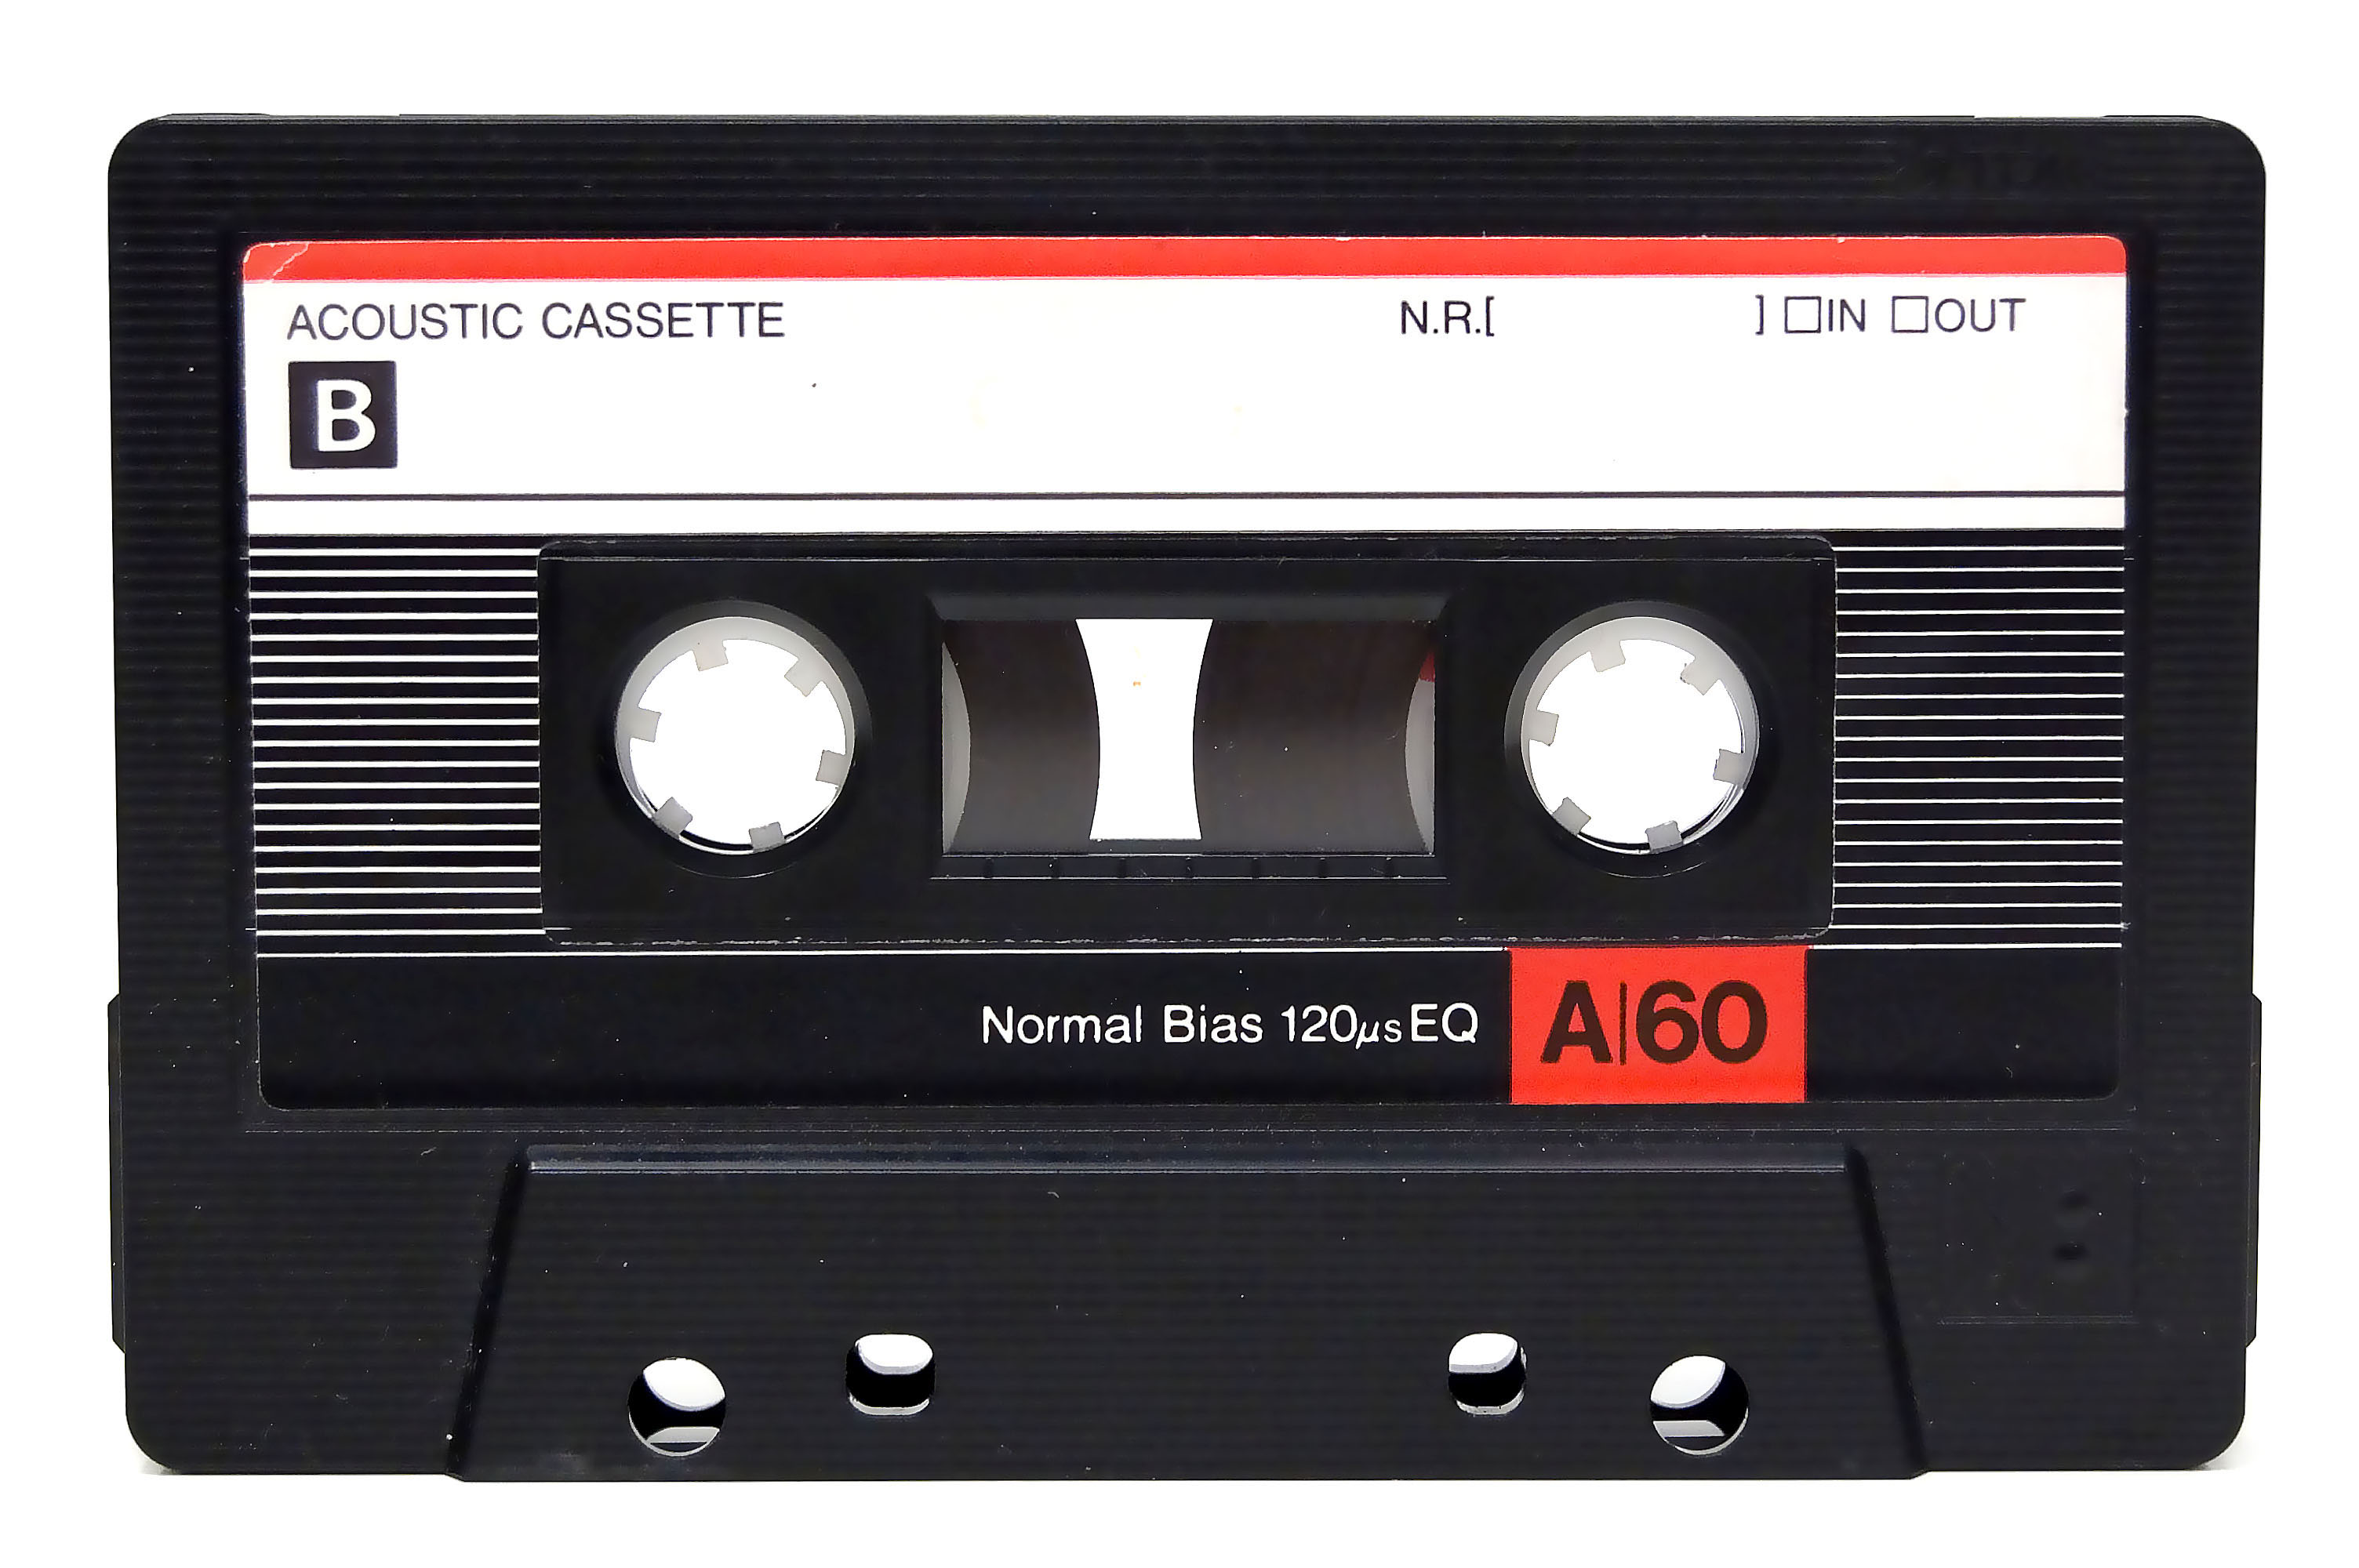
\includegraphics[height=5.5cm]{img/cassette}
\end{minipage}
\end{textblock*}
\end{frame}

\begin{frame}{\ \ \ ALGOL-60 и далее}
\setstretch{1.2}
\begin{textblock*}{\framewidth}(0.8cm,1.5cm)
  \begin{columns}[onlytextwidth,t]
    \begin{column}{0.5\textwidth}
      \centering
      
\includegraphics[height=6.8cm,valign=t]{img/algorithm}
    \end{column}
    \begin{column}{0.5\textwidth}
    Структурное и процедурное программирование
    \end{column}
  \end{columns}
\end{textblock*}
\end{frame}

\begin{frame}{\ \ \ Корень всех зол (нет, не goto)}
\setstretch{1.2}
\begin{textblock*}{\framewidth-0.5cm}(1.2cm,1.5cm)
  \begin{columns}[onlytextwidth,t]
    \begin{column}{0.5\textwidth}
      Как C-программист под DSP пишет на C{\lserif\#}?\\
      {\small В C{\lserif\#} нет goto, но это не беда!}
    \end{column}
    \begin{column}{0.5\textwidth}
      \centering
      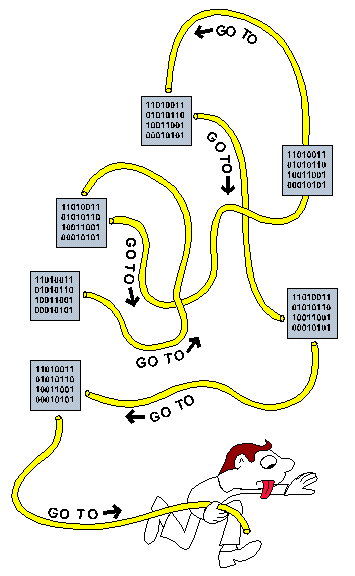
\includegraphics[height=6.8cm,valign=t]{img/spaghetti.png}
    \end{column}
  \end{columns}
\end{textblock*}
\end{frame}

\begin{frame}{\ \ \ Зачем нужно OOP?}
\setstretch{1.2}
\begin{textblock*}{\framewidth-0.8cm}(0.5cm,1.5cm)
\begin{itemize}
  \item Инкапсуляция, наследование, полиморфизм!
  \item Пенсия Гради Буча
\end{itemize}
\end{textblock*}
\end{frame}

\begin{frame}{\ \ \ Зачем на самом деле OOP?}
\setstretch{1.2}
\begin{textblock*}{\framewidth-0.8cm}(0.5cm,1.5cm)
\begin{itemize}
  \item Инкапсуляция, наследование, полиморфизм!
  \item Пенсия Гради Буча
  \item Кошелек Миллера (спасибо Григорию Петрову)
  \item Закон Деметры
  \item SOLID
\end{itemize}
\end{textblock*}
\end{frame}

\begin{frame}{\ \ \ SOLID}
\setstretch{1.2}
\begin{textblock*}{\framewidth-0.8cm}(0.5cm,1.5cm)
\begin{itemize}
  \item Single responsibility principle
\end{itemize}
\end{textblock*}
\end{frame}

\begin{frame}{\ \ \ SOLID}
\setstretch{1.2}
\begin{textblock*}{\framewidth-0.8cm}(0.5cm,1.5cm)
\begin{itemize}
  \item Single responsibility principle
  \item Open/closed principle
\end{itemize}
\end{textblock*}
\end{frame}

\begin{frame}{\ \ \ SOLID}
\setstretch{1.2}
\begin{textblock*}{\framewidth-0.8cm}(0.5cm,1.5cm)
\begin{itemize}
  \item Single responsibility principle
  \item Open/closed principle
  \item Liskov substitution principle
\end{itemize}
\end{textblock*}
\end{frame}

\begin{frame}{\ \ \ SOLID}
\setstretch{1.2}
\begin{textblock*}{\framewidth-0.8cm}(0.5cm,1.5cm)
\begin{itemize}
  \item Single responsibility principle
  \item Open/closed principle
  \item Liskov substitution principle
  \item Interface segregation principle
\end{itemize}
\end{textblock*}
\end{frame}

\begin{frame}{\ \ \ SOLID}
\setstretch{1.2}
\begin{textblock*}{\framewidth-0.8cm}(0.5cm,1.5cm)
\begin{itemize}
  \item Single responsibility principle
  \item Open/closed principle
  \item Liskov substitution principle
  \item Interface segregation principle
  \item Dependency inversion principle
\end{itemize}
\end{textblock*}
\end{frame}

\begin{frame}{\ \ \ Что-то пошло не так}
\setstretch{1.2}
\begin{textblock*}{\framewidth}(0.8cm,1.5cm)
Objects have failed* (OOPSLA 2002)\\
{\small * на самом деле нет}
\begin{minipage}{\textwidth}
  \centering
  
\includegraphics[height=5.5cm]{img/fail}
\end{minipage}
\end{textblock*}
\end{frame}

\begin{frame}{\ \ \ 2002+15}
\setstretch{1.2}
\begin{textblock*}{\framewidth}(0.8cm,1.5cm)
Python - lingua franca индустрии\\
{\small В Python есть всё}
\begin{minipage}{\textwidth}
  \centering
  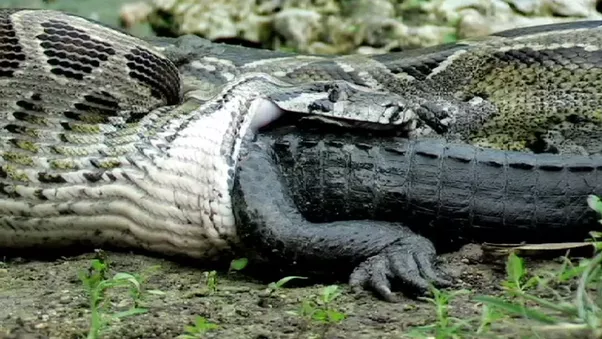
\includegraphics[height=5.5cm]{img/python}
\end{minipage}
\end{textblock*}
\end{frame}

\begin{frame}{\ \ \ В Python есть всё}
\setstretch{1.2}
\begin{textblock*}{\framewidth}(0.8cm,1.5cm)
Зачем тогда что-то еще?\\
\begin{minipage}{\textwidth}
  \centering
  
\includegraphics[height=5.5cm]{img/Conspiracy-Keanu}
\end{minipage}
\end{textblock*}
\end{frame}

\begin{frame}{\ \ \ Отнять и поделить}
\setstretch{1.2}
\begin{textblock*}{\framewidth}(0.8cm,1.5cm)
Почему не декриминализуют легкие наркотики?\\
\begin{minipage}{\textwidth}
  \centering
  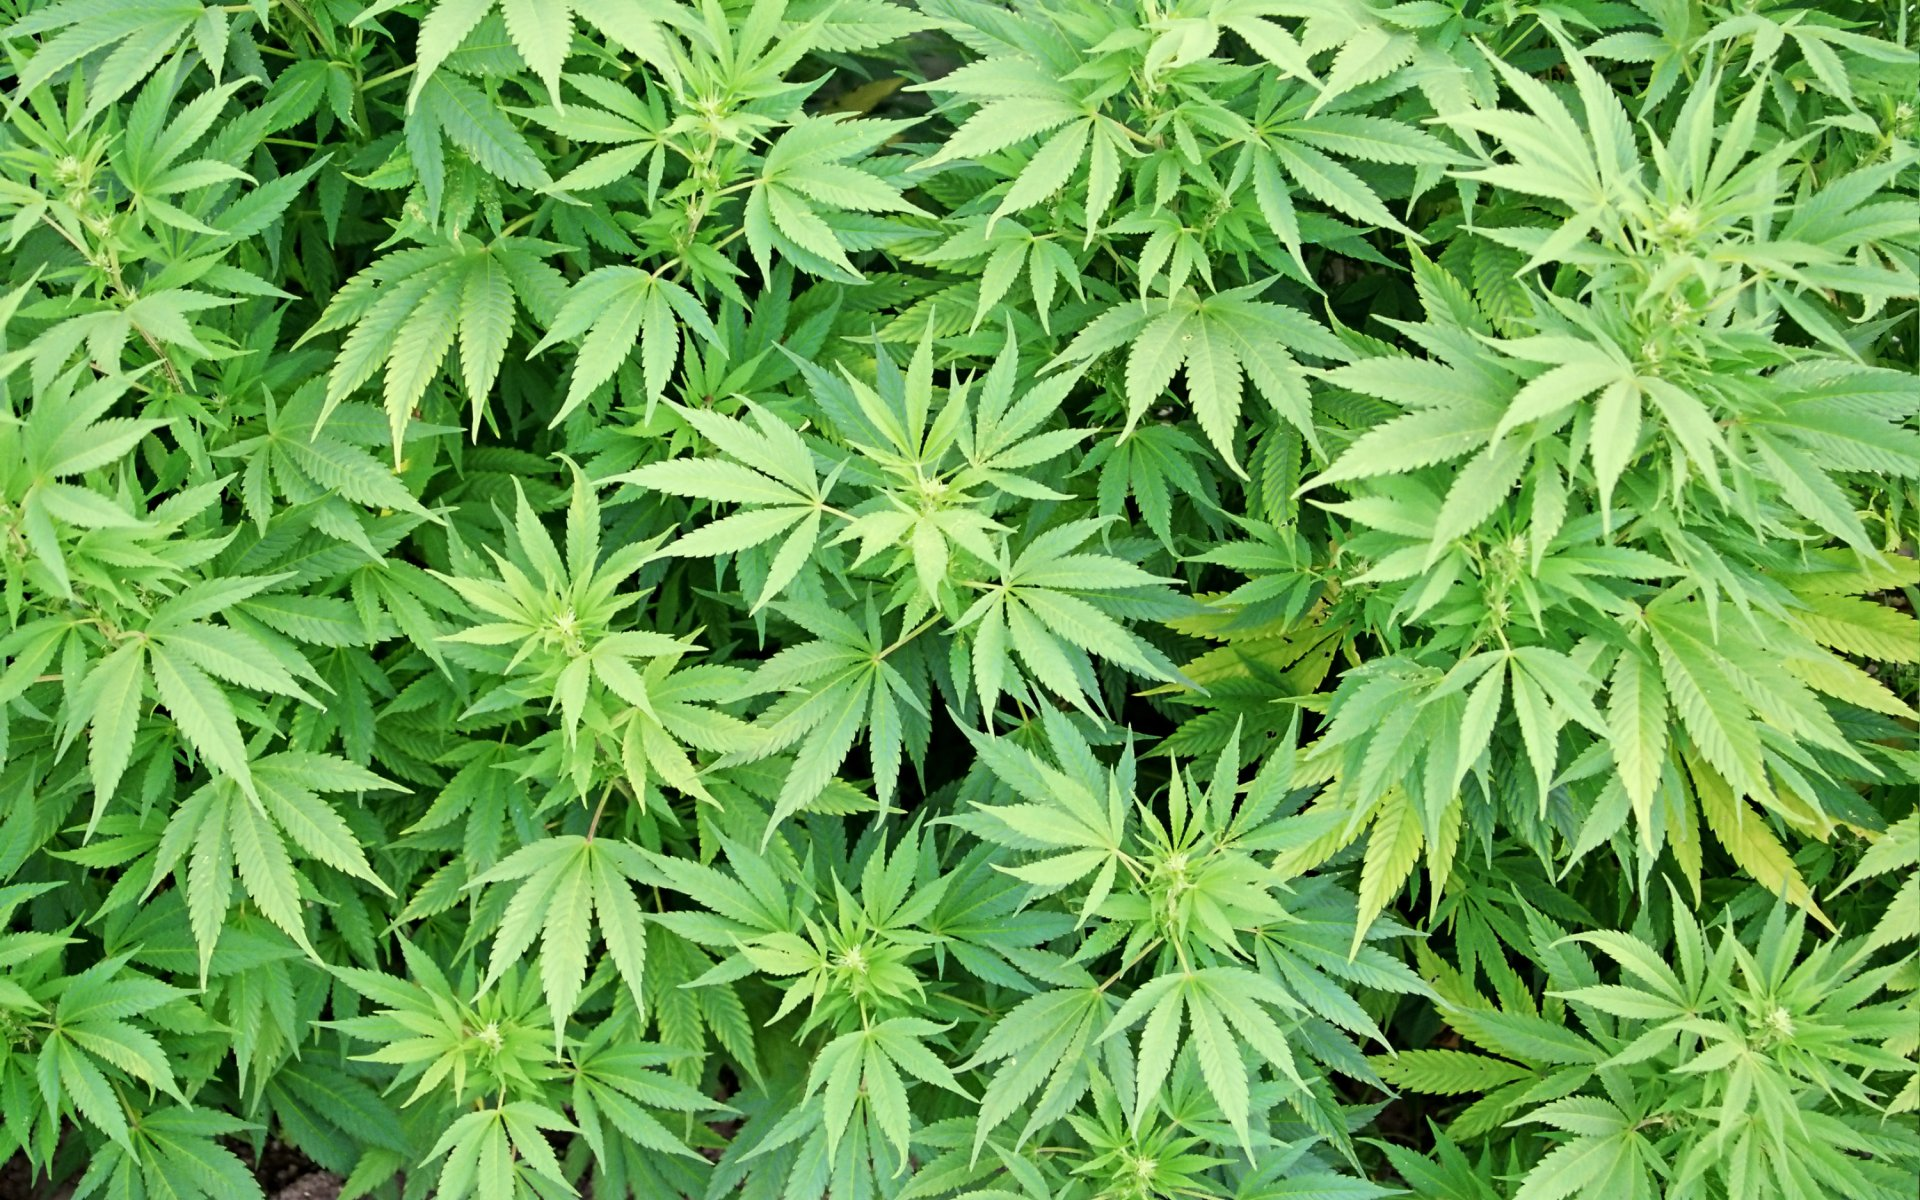
\includegraphics[height=5.5cm]{img/weed}
\end{minipage}
\end{textblock*}
\end{frame}

\begin{frame}{\ \ \ Хороший Язык Будущего}
\setstretch{1.2}
\begin{textblock*}{\framewidth-0.8cm}(0.5cm,1.5cm)
\begin{itemize}
  \item Строгая типизация (PHP и JS - плохие)
\end{itemize}
\end{textblock*}
\end{frame}

\begin{frame}{\ \ \ Хороший Язык Будущего}
\setstretch{1.2}
\begin{textblock*}{\framewidth-0.8cm}(0.5cm,1.5cm)
\begin{itemize}
  \item Строгая типизация (PHP и JS - плохие)
  \item (Опциональная) статическая типизация
\end{itemize}
\end{textblock*}
\end{frame}

\begin{frame}{\ \ \ Опциональная типизация}
\setstretch{1.2}
\begin{textblock*}{\framewidth-0.8cm}(0.5cm,1.5cm)
\begin{itemize}
  \item PHP: type declarations, 5.0 => 7.0
  \item Python: type hints, PEP-484
  \item Python: mypy
\end{itemize}
\end{textblock*}
\end{frame}

\begin{frame}{\ \ \ Статические анализаторы}
\setstretch{1.2}
\begin{textblock*}{\framewidth-0.8cm}(0.5cm,1.5cm)
\begin{itemize}
  \item mypy - статический анализатор кода
\end{itemize}
\end{textblock*}
\end{frame}

\begin{frame}{\ \ \ Статические анализаторы}
\setstretch{1.2}
\begin{textblock*}{\framewidth-0.8cm}(0.5cm,1.5cm)
\begin{itemize}
  \item mypy - статический анализатор кода
  \item статический анализатор работает до запуска программы
\end{itemize}
\end{textblock*}
\end{frame}

\begin{frame}{\ \ \ Статические анализаторы}
\setstretch{1.2}
\begin{textblock*}{\framewidth-0.8cm}(0.5cm,1.5cm)
\begin{itemize}
  \item mypy - статический анализатор кода
  \item статический анализатор работает до запуска программы
  \item статический анализатор обобщает идею статической типизации
\end{itemize}
\end{textblock*}
\end{frame}

\begin{frame}{\ \ \ Анализаторы разных языков}
\setstretch{1.2}
\begin{textblock*}{\framewidth-0.8cm}(0.5cm,1.5cm)
\begin{itemize}
  \item Ruby: RuboCop
  \item Perl: Perl::Critic
  \item Python: Coala, Pylama, mypy
  \item PHP: PHPLint, PHP Mess Detector
\end{itemize}
\end{textblock*}
\end{frame}

\begin{frame}{\ \ \ Static Analysis Symposium}
\setstretch{1.2}
\begin{textblock*}{\framewidth}(0.5cm,1.5cm)
\begin{itemize}
  \item Научная конференция
  \item Проходила уже 23 раза
  \item 23 сборника статей примерно по 400 страниц
\end{itemize}
\begin{minipage}{\textwidth}
  \centering
  
\includegraphics[height=4.0cm]{img/slozhna}
\end{minipage}
\end{textblock*}
\end{frame}

\begin{frame}{\ \ \ Хороший Язык Будущего}
\setstretch{1.2}
\begin{textblock*}{\framewidth-0.8cm}(0.5cm,1.5cm)
\begin{itemize}
  \item Строгая типизация (PHP и JS - плохие)
  \item (Опциональная) статическая типизация
  \item Package/vendoring manager
\end{itemize}
\end{textblock*}
\end{frame}

\begin{frame}{\ \ \ Package managers}
\setstretch{1.2}
\begin{textblock*}{\framewidth-0.8cm}(0.5cm,1.5cm)
\begin{itemize}
  \item PHP: Composer
  \item Python: pip
  \item Perl: cpanminus
  \item Ruby: bundler
\end{itemize}
\end{textblock*}
\end{frame}

\begin{frame}{\ \ \ Хороший Язык Будущего}
\setstretch{1.2}
\begin{textblock*}{\framewidth-0.8cm}(0.5cm,1.5cm)
\begin{itemize}
  \item {\color{gray}{Строгая типизация (PHP и JS - плохие)}}
  \item {\color{gray}{(Опциональная) статическая типизация}}
  \item {\color{gray}{Package/vendoring manager}}
\end{itemize}
\end{textblock*}
\end{frame}

\begin{frame}{\ \ \ Хороший Язык Будущего}
\setstretch{1.2}
\begin{textblock*}{\framewidth-0.8cm}(0.5cm,1.5cm)
\begin{itemize}
  \item {\color{gray}{Строгая типизация (PHP и JS - плохие)}}
  \item {\color{gray}{(Опциональная) статическая типизация}}
  \item {\color{gray}{Package/vendoring manager}}
  \item Метапрограммирование
\end{itemize}
\end{textblock*}
\end{frame}

\begin{frame}{\ \ \ Хороший Язык Будущего}
\setstretch{1.2}
\begin{textblock*}{\framewidth-0.8cm}(0.5cm,1.5cm)
\begin{itemize}
  \item {\color{gray}{Строгая типизация (PHP и JS - плохие)}}
  \item {\color{gray}{(Опциональная) статическая типизация}}
  \item {\color{gray}{Package/vendoring manager}}
  \item Метапрограммирование
  \item Иммутабельность
\end{itemize}
\end{textblock*}
\end{frame}

\begin{frame}{\ \ \ Иммутабельность}
\setstretch{1.2}
\begin{textblock*}{\framewidth}(0.8cm,1.5cm)
Доклад Боба Ипполито в 2014-м\\
{\small верен и в 2017-м}
\begin{minipage}{\textwidth}
  \centering
  
\includegraphics[height=6.0cm]{img/bobippolito}
\end{minipage}
\end{textblock*}
\end{frame}

\begin{frame}{\ \ \ Хороший Язык Будущего}
\setstretch{1.2}
\begin{textblock*}{\framewidth-0.8cm}(0.5cm,1.5cm)
\begin{itemize}
  \item {\color{gray}{Строгая типизация (PHP и JS - плохие)}}
  \item {\color{gray}{(Опциональная) статическая типизация}}
  \item {\color{gray}{Package/vendoring manager}}
  \item Метапрограммирование
  \item Иммутабельность
  \item Null-safety
\end{itemize}
\end{textblock*}
\end{frame}

\begin{frame}{\ \ \ Метапрограммирование}
\setstretch{1.2}
\begin{textblock*}{\framewidth}(0.5cm,1.5cm)
\begin{itemize}
  \item Было в C - \#ifdef
\end{itemize}
\begin{minipage}{\textwidth}
  \centering
  
\includegraphics[height=6.0cm]{img/pain}
\end{minipage}
\end{textblock*}
\end{frame}

\begin{frame}{\ \ \ Метапрограммирование}
\setstretch{1.2}
\begin{textblock*}{\framewidth}(0.5cm,1.5cm)
\begin{itemize}
  \item Было в C - \#ifdef
  \item Было в Java - аннотации
\end{itemize}
\begin{minipage}{\textwidth}
  \centering
  
\includegraphics[height=5.2cm]{img/happiness}
\end{minipage}
\end{textblock*}
\end{frame}

\begin{frame}{\ \ \ Метапрограммирование}
\setstretch{1.2}
\begin{textblock*}{\framewidth}(0.5cm,1.5cm)
\begin{itemize}
  \item Было в C - \#ifdef
  \item Было в Java - аннотации
  \item Было в LISP - макросы
\end{itemize}
\begin{minipage}{\textwidth}
  \centering
  
\includegraphics[height=4.5cm]{img/megamind}
\end{minipage}
\end{textblock*}
\end{frame}

\begin{frame}{\ \ \ Сферический в вакууме}
\setstretch{1.2}
\begin{textblock*}{\framewidth}(0.5cm,1.5cm)
\begin{itemize}
  \item Языку нужна среда исполнения
\end{itemize}
\end{textblock*}
\end{frame}

\begin{frame}{\ \ \ Сферический в вакууме}
\setstretch{1.2}
\begin{textblock*}{\framewidth}(0.5cm,1.5cm)
\begin{itemize}
  \item Языку нужна среда исполнения
  \item JVM
\end{itemize}
\end{textblock*}
\end{frame}

\begin{frame}{\ \ \ Сферический в вакууме}
\setstretch{1.2}
\begin{textblock*}{\framewidth}(0.5cm,1.5cm)
\begin{itemize}
  \item Языку нужна среда исполнения
  \item JVM
  \item V8
\end{itemize}
\end{textblock*}
\end{frame}

\begin{frame}{\ \ \ Сферический в вакууме}
\setstretch{1.2}
\begin{textblock*}{\framewidth}(0.5cm,1.5cm)
\begin{itemize}
  \item Языку нужна среда исполнения
  \item JVM
  \item V8
  \item BEAM
\end{itemize}
\end{textblock*}
\end{frame}

\begin{frame}{\ \ \ Сферический в вакууме}
\setstretch{1.2}
\begin{textblock*}{\framewidth}(0.5cm,1.5cm)
\begin{itemize}
  \item Языку нужна среда исполнения
  \item JVM
  \item V8
  \item BEAM
  \item Golang runtime (not a VM, but...)
\end{itemize}
\end{textblock*}
\end{frame}

\begin{frame}{\ \ \ A quest for my next PL}
\setstretch{1.2}
\begin{textblock*}{\framewidth}(0.8cm,1.5cm)
  \href{https://goo.gl/MS1UfB}{\color{blue}{https://goo.gl/MS1UfB}}\\
\begin{minipage}{\textwidth}
  \centering
  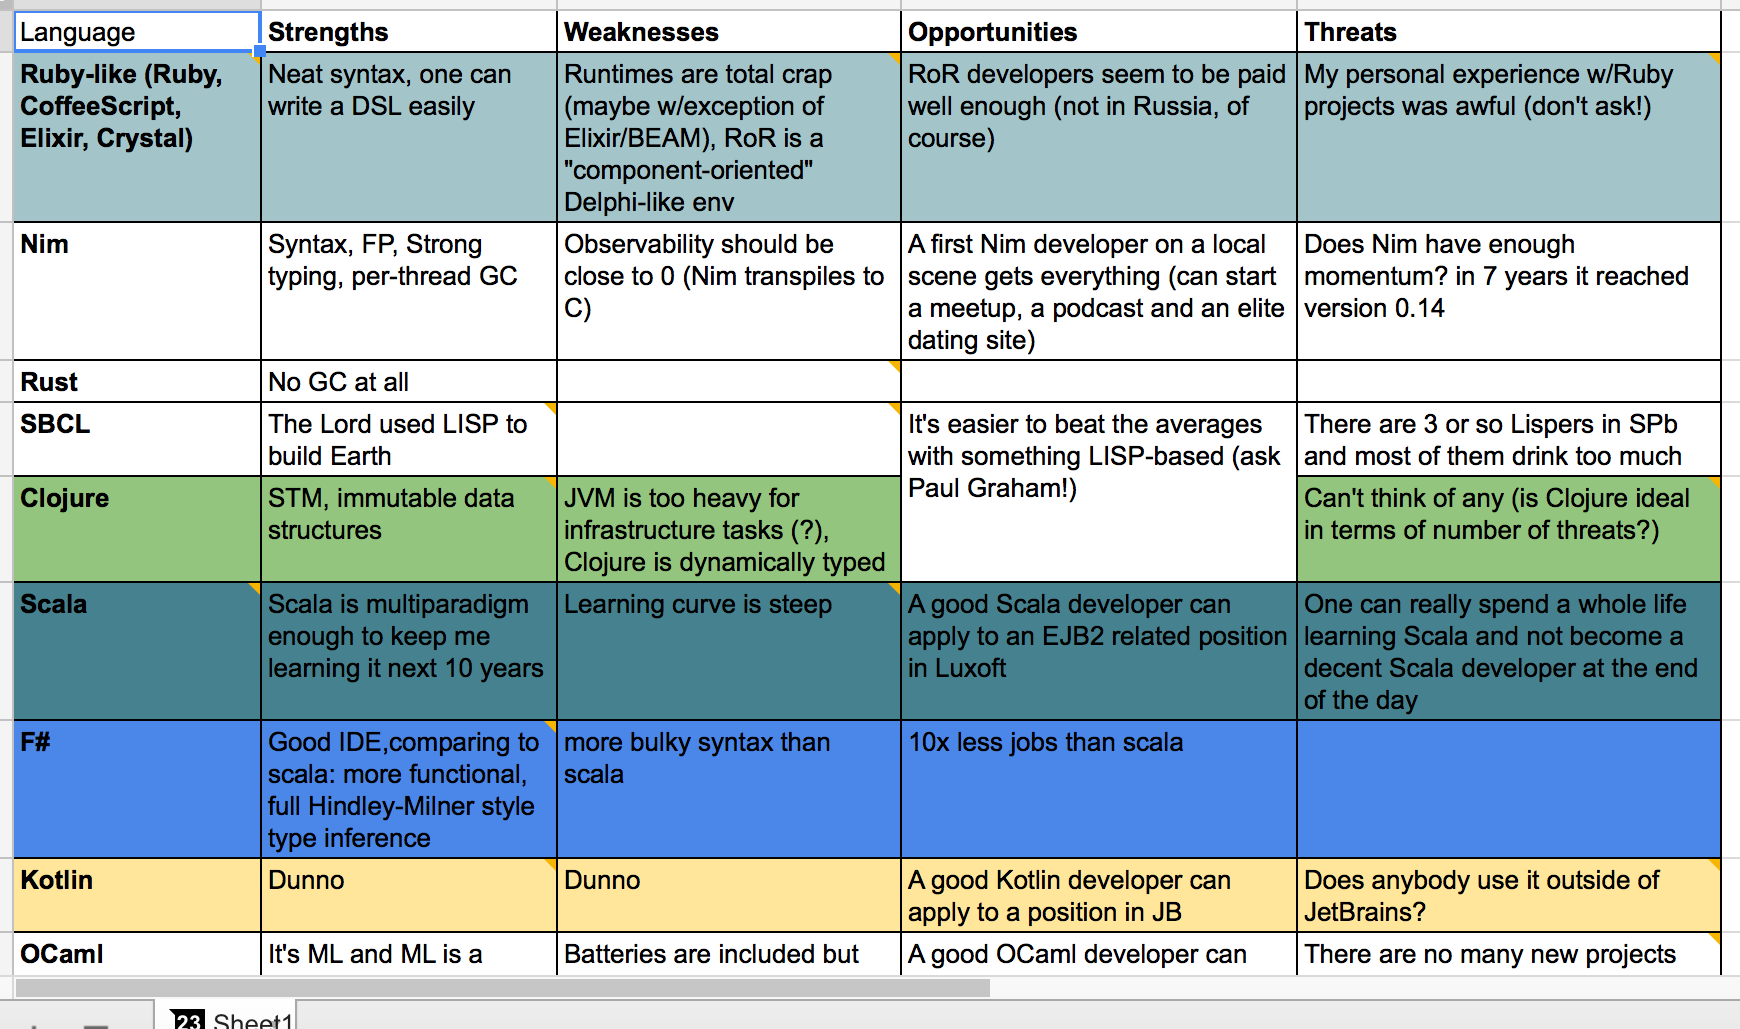
\includegraphics[height=6.5cm]{img/quest.png}
\end{minipage}
\end{textblock*}
\end{frame}

\begin{frame}{\ \ \ Буду гиперполиглотом}
\setstretch{1.2}
\begin{textblock*}{\framewidth}(0.8cm,1.5cm)
  \href{http://hyperpolyglot.org}{\color{blue}{http://hyperpolyglot.org}}\\
\begin{minipage}{\textwidth}
  \centering
  
\includegraphics[height=6.8cm]{img/malloc}
\end{minipage}
\end{textblock*}
\end{frame}

\begin{frame}{\ \ \ Почему не Golang?}
\setstretch{1.2}
\begin{textblock*}{\framewidth-0.8cm}(0.5cm,1.5cm)
\begin{itemize}
  \item Очень простой: 25 ключевых слов
\end{itemize}
\end{textblock*}
\end{frame}

\begin{frame}{\ \ \ Почему не Golang?}
\setstretch{1.2}
\begin{textblock*}{\framewidth-0.8cm}(0.5cm,1.5cm)
\begin{itemize}
  \item Очень простой: 25 ключевых слов
  \item Нет метапрограммирования
\end{itemize}
\end{textblock*}
\end{frame}

\begin{frame}{\ \ \ Почему не Golang?}
\setstretch{1.2}
\begin{textblock*}{\framewidth-0.8cm}(0.5cm,1.5cm)
\begin{itemize}
  \item Очень простой: 25 ключевых слов
  \item Нет метапрограммирования
  \item Нет иммутабельности
\end{itemize}
\end{textblock*}
\end{frame}

\begin{frame}{\ \ \ Почему не Golang?}
\setstretch{1.2}
\begin{textblock*}{\framewidth-0.8cm}(0.5cm,1.5cm)
\begin{itemize}
  \item Очень простой: 25 ключевых слов
  \item Нет метапрограммирования
  \item Нет иммутабельности
  \item Нет null-safety
\end{itemize}
\end{textblock*}
\end{frame}

\begin{frame}{\ \ \ Почему не Golang?}
\setstretch{1.2}
\begin{textblock*}{\framewidth-0.8cm}(0.5cm,1.5cm)
\begin{itemize}
  \item Очень простой: 25 ключевых слов
  \item Нет метапрограммирования
  \item Нет иммутабельности
  \item Нет null-safety
  \item Из Golang легко сделать Python
\end{itemize}
\end{textblock*}
\end{frame}

\begin{frame}{\ \ \ Почему не Golang?}
\setstretch{1.2}
\begin{textblock*}{\framewidth-0.8cm}(0.5cm,1.5cm)
\begin{itemize}
  \item Очень простой: 25 ключевых слов
  \item Нет метапрограммирования
  \item Нет иммутабельности
  \item Нет null-safety
  \item Из Golang легко сделать Python
  \item С вендорингом какая-то боль
\end{itemize}
\end{textblock*}
\end{frame}

\begin{frame}{\ \ \ Что реально успел?}
\setstretch{1.2}
\begin{textblock*}{\framewidth-0.8cm}(0.5cm,1.5cm)
\begin{itemize}
  \item Clojure: dynamic, strong
  \item Elixir: dynamic, strong
  \item Nim: static, strong, null-unsafe
  \item Rust: static, strong, null-safe
\end{itemize}
\end{textblock*}
\end{frame}

\begin{frame}{\ \ \ Как ощущения?}
\setstretch{1.2}
\begin{textblock*}{\framewidth-0.8cm}(0.5cm,1.5cm)
Use libraries, not frameworks!
\begin{itemize}
  \item {\color{gray}{Clojure: dynamic, strong}}
  \item {\color{gray}{Elixir: dynamic, strong}}
  \item Nim: static, strong, null-unsafe
  \item Rust: static, strong, null-safe
\end{itemize}
\end{textblock*}
\end{frame}

\begin{frame}{\ \ \ Use libraries, not frameworks!}
\setstretch{1.2}
\begin{textblock*}{\framewidth-0.8cm}(0.5cm,1.5cm)
\begin{itemize}
  \item Везде генерируется scaffolding    
  \item Везде есть порт Sinatra
  \item Везде есть ORM tool
\end{itemize}
\end{textblock*}
\end{frame}

\begin{frame}{\ \ \ Haskell}
\setstretch{1.2}
\begin{textblock*}{\framewidth}(0.8cm,1.5cm)
Как открыть ВАЗ 2101 без ключа?\\
{\small (Гораздо легче, чем пройти курс по Haskell*)}
\begin{minipage}{\textwidth}
  \centering
  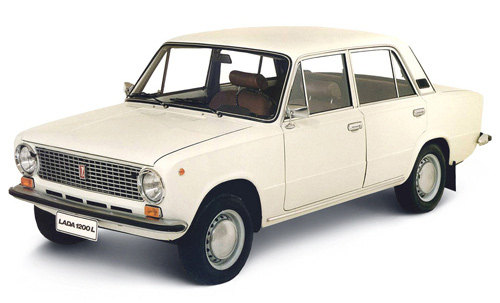
\includegraphics[height=5.5cm]{img/lada_2101_1.jpg}
\end{minipage}
\end{textblock*}
\end{frame}

\begin{frame}{\ \ \ Выводы}
\setstretch{1.2}
\begin{textblock*}{\framewidth-0.8cm}(0.5cm,1.5cm)
\begin{itemize}
  \item Я не знаю, что будет дальше
  \item Я не знаю, какой язык лучший
  \item Поэтому писать надо на всем
  \item Но, если можете, не пишите на COBOL
\end{itemize}
\end{textblock*}
\end{frame}

\begin{frame}{\ \ \ Вопросы, пожалуйста?}
\setstretch{1.2}
\begin{textblock*}{\framewidth-0.8cm}(0.5cm,1.5cm)
\begin{itemize}
  \item ...?
  \item ...?
  \item ...?
\end{itemize}
\end{textblock*}
\end{frame}

\begin{frame}{\ \ \ That's all, folks!}
\setstretch{1.2}
\begin{textblock*}{\framewidth-0.8cm}(0.5cm,1.5cm)
\begin{itemize}
  \item \href{mailto:alex@gitinsky.com}{\color{blue}{alex@gitinsky.com}}
  \item \href{https://telegram.me/lhommequipleure}{\color{blue}{https://telegram.me/lhommequipleure}}
\end{itemize}
\end{textblock*}
\end{frame}
\end{Large}

\end{document}